\section{Model-driven Development}
\begin{frame}{Model-driven Software Development (MDD)}
	\framesubtitle{Overview}

	\begin{columns}[T]
		\begin{column}{.48\textwidth}
			\centering
			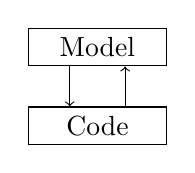
\begin{tikzpicture}[every node/.style={draw, minimum width = 50}]
				\node(model){Model};
				\node[below of=model](code){Code};
				\draw[->, transform canvas={xshift=-10}](model) -- (code);
				\draw[->, transform canvas={xshift= 10}](code) -- (model);
			\end{tikzpicture}
		\end{column}
		\begin{column}{.48\textwidth}
			\centering	
			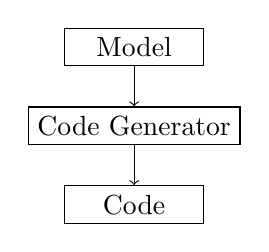
\begin{tikzpicture}[every node/.style={draw, minimum width = 50}]
				\node(model){Model};
				\node[below of=model](generator){Code Generator};
				\node[below of=generator](code){Code};
				\draw[->](model) -- (generator);
				\draw[->](generator) -- (code);
			\end{tikzpicture}
		\end{column}
	\end{columns}
	
	Advantages
	
	\begin{itemize}
		\item Better abstraction
		\item \textbf{Models are easier to check for logical errors}
		\item Models are easier to understand for non-programmers
	\end{itemize}
\end{frame}

\begin{frame}{}
	Our use of MDD
	
	In combination with an iterative workflow
	
	Problem division
	
	\begin{tikzpicture}
	
		\node(design){Design};
		
		\node[right of=design](model){Model};
		
		\node[below right of=design](implementation){Implementation}
		
		\node[right of=implementation](code){Code}
		
		\node[left of=implementation](evaluation){Evaluation}
	
	\end{tikzpicture}
	
\end{frame}

\section{Model checking}
\begin{frame}{Model checking}
\framesubtitle{UUPAAL}

	\begin{block}{Description}
		``Uppaal is an integrated tool environment for modeling, validation and verification of real-time systems modeled as networks of timed automata, extended with data types (bounded integers, arrays, etc.).''\footnote{http://www.uppaal.org/}
	\end{block}
	
\end{frame}